\documentclass[a4paper,oneside,11pt]{book}

% Package yang diperlukan
\usepackage{graphicx}
\usepackage{titling}
\usepackage{geometry}
\usepackage{listings}
\usepackage{xcolor}
\usepackage{float}
\usepackage{hyperref}
\usepackage{indentfirst}
\usepackage{longtable}
\usepackage{array}

% Pengaturan margin
\geometry{
    left=3cm,
    right=2.5cm,
    top=3cm,
    bottom=3cm
}
% Pengaturan untuk kode HTML
\definecolor{codegreen}{rgb}{0,0.6,0}
\definecolor{codegray}{rgb}{0.5,0.5,0.5}
\definecolor{codepurple}{rgb}{0.58,0,0.82}
\definecolor{backcolour}{rgb}{0.95,0.95,0.92}

\lstdefinestyle{javastyle}{
    language=Java,
    backgroundcolor=\color{backcolour},
    commentstyle=\color{codegreen},
    keywordstyle=\color{blue}\bfseries,
    numberstyle=\tiny\color{codegray},
    stringstyle=\color{orange},
    basicstyle=\ttfamily\footnotesize,
    breakatwhitespace=false,
    breaklines=true,
    captionpos=b,
    keepspaces=true,
    numbers=left,
    numbersep=5pt,
    showspaces=false,
    showstringspaces=false,
    showtabs=false,
    tabsize=2,
    frame=single
}


\title{Laporan Praktikum \\ Praktikum Pengujian Perangkat Lunak\\
Pertemuan 1\\
 Unit Test \& Assertion}
\author{Nama Mahasiswa: Januarsyah Akbar (24/535846/SV/24314)}
\date{\today}

\begin{document}

% Halaman judul
\begin{titlingpage}
\begin{center}
\vspace{4cm}
\begin{huge} 
\textbf{\thetitle} \\
\end{huge}
\vspace{2cm}

\includegraphics[height=8cm]{lambang ugm.png}\\
\begin{Large}
\vspace{4cm}
\theauthor\\
Kelas B2 \\
\end{Large}
\begin{large}
Dosen Pengampu: Divi Galih Prasetyo Putri, S.Kom., M.Kom., Ph.D.\\
\end{large}
\vspace{2cm}
\thedate
\end{center}
\end{titlingpage}

% Daftar Isi
\tableofcontents
\newpage
\chapter{Tujuan Praktikum}
\begin{enumerate}
    \item Mahasiswa mampu memahami unit testing
    \item Mahasiswa mampu menggunakan JUnit
    \item Mahasiswa memahami konsep assertion
    \item Mahasiswa mampu mengimplementasikan assertion pada pengujian unit
\end{enumerate}
\chapter{Langkah Praktikum}
\section{Unit Test}
\begin{enumerate}
    \item Buka IDE yang digunakan, seperti IntelliJ IDEA atau Eclipse.
    \item Buat proyek Java baru dengan Build system Maven (pada laporan ini menggunakan IntelliJ IDEA, dengan JDK versi 23).
    % insert image of creating new project
    \figure[H]
        \centering
        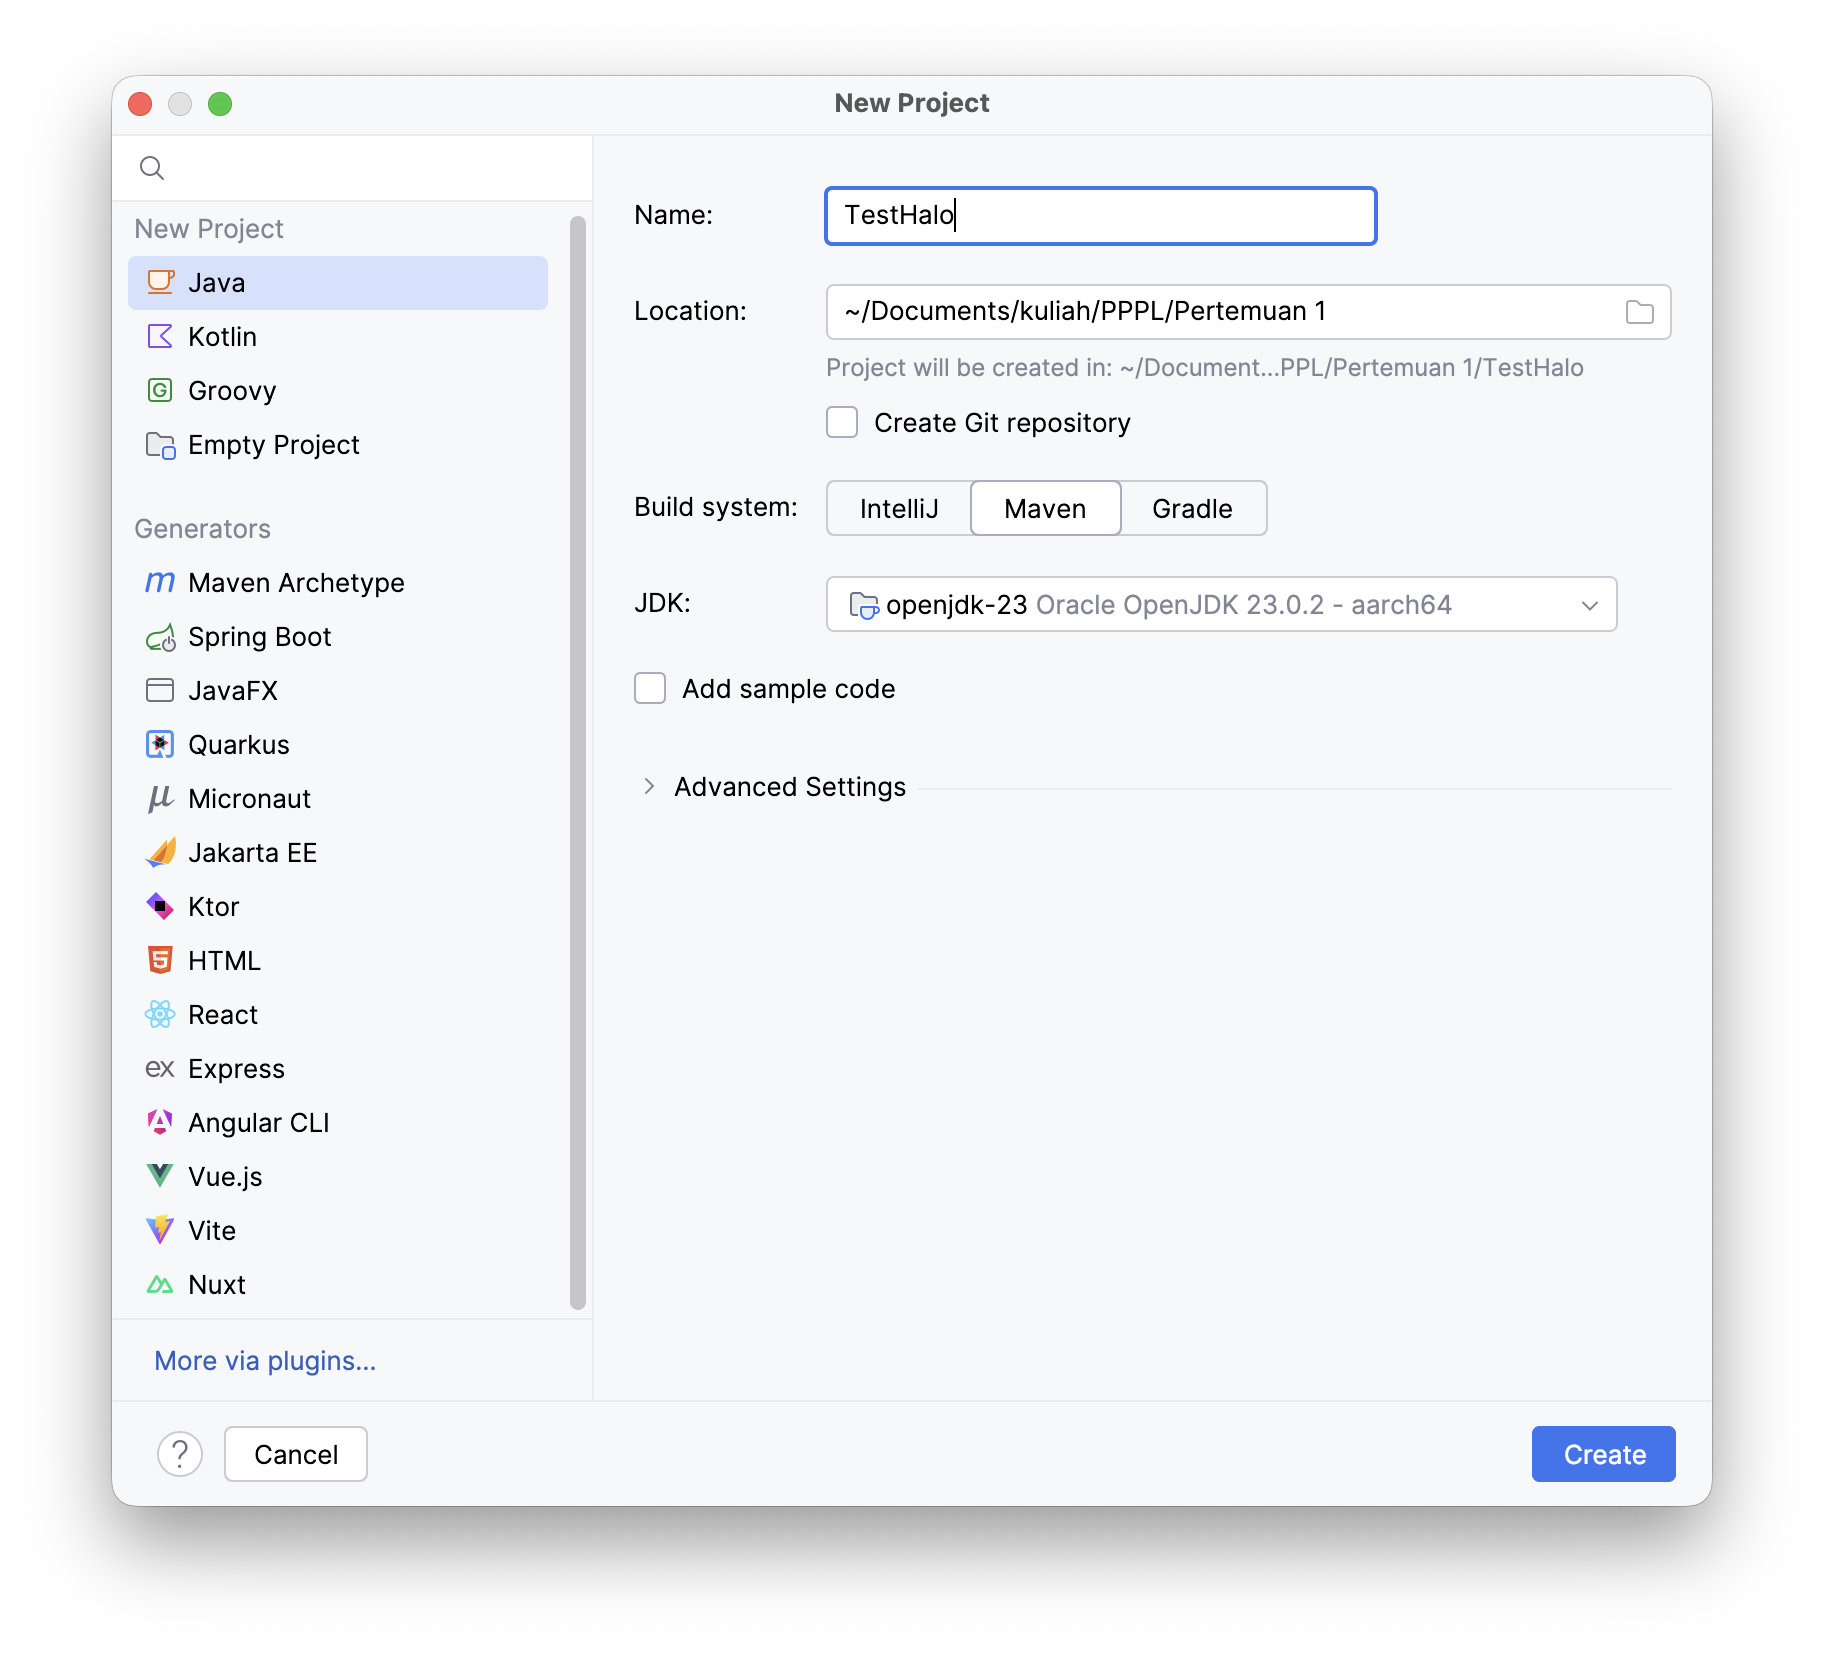
\includegraphics[width=0.7\textwidth]{newproject.png}
        \caption{Membuat Proyek Baru di IntelliJ IDEA}
    \endfigure
    \item Tambahkan dependensi JUnit pada file \texttt{pom.xml} untuk menggunakan framework JUnit dalam proyek. Kunjungi halaman berikut untuk menambahkan JUnit secara manual:

    \url{https://mvnrepository.com/artifact/org.junit.jupiter/junit-jupiter/5.13.4}

    Pilih Maven dengan Scope Test dan salin kode dependensi yang diberikan. Paste kodet tadi ke dalam tag <dependencies> di file \texttt{pom.xml} seperti berikut:
    \\
\begin{lstlisting}[style=javastyle,language=XML,caption=Menambahkan Dependensi JUnit di pom.xml]
<dependencies>
<!-- Source: https://mvnrepository.com/artifact/org.junit.jupiter/junit-jupiter -->
<dependency>
    <groupId>org.junit.jupiter</groupId>
    <artifactId>junit-jupiter</artifactId>
    <version>5.13.4</version>
    <scope>test</scope>
</dependency>
</dependencies>
\end{lstlisting}
    \item Setelah menambahkan dependensi jalankan shortcut Command + Shift + I untuk sync Maven.
    \item Buat class biasa, contoh return "hello world" pada class tersebut.
\begin{lstlisting}[style=javastyle,caption=Contoh Class Java Sederhana]
// location: src/main/java/Hello.java
public class Hello {
    public String helloWorld()
    {
        return "hello world";
    }
}
\end{lstlisting}
    \item Buat class test pada folder \texttt{src/test/java} dengan nama yang sama dengan class yang akan di test, namun dengan tambahan suffix \texttt{Test}.
\begin{lstlisting}[style=javastyle,caption=Contoh Class Test Java Sederhana]
// location: src/test/java/HelloTest.java
import static org.junit.jupiter.api.Assertions.*;
import org.junit.jupiter.api.Test;
public class HelloTest {
    @Test
    public void testHelloWorld() {
        Hello hello = new Hello();
        String result = hello.helloWorld();
        assertEquals("hello world", result);
    }
}
\end{lstlisting}
    \item Jalankan class test untuk memastikan bahwa unit test berjalan dengan benar.   
    \item Jika semua langkah di atas dilakukan dengan benar, maka hasil dari unit test akan menunjukkan bahwa semua test berhasil (green bar) seperti gambar berikut:
    \figure[H]
        \centering
        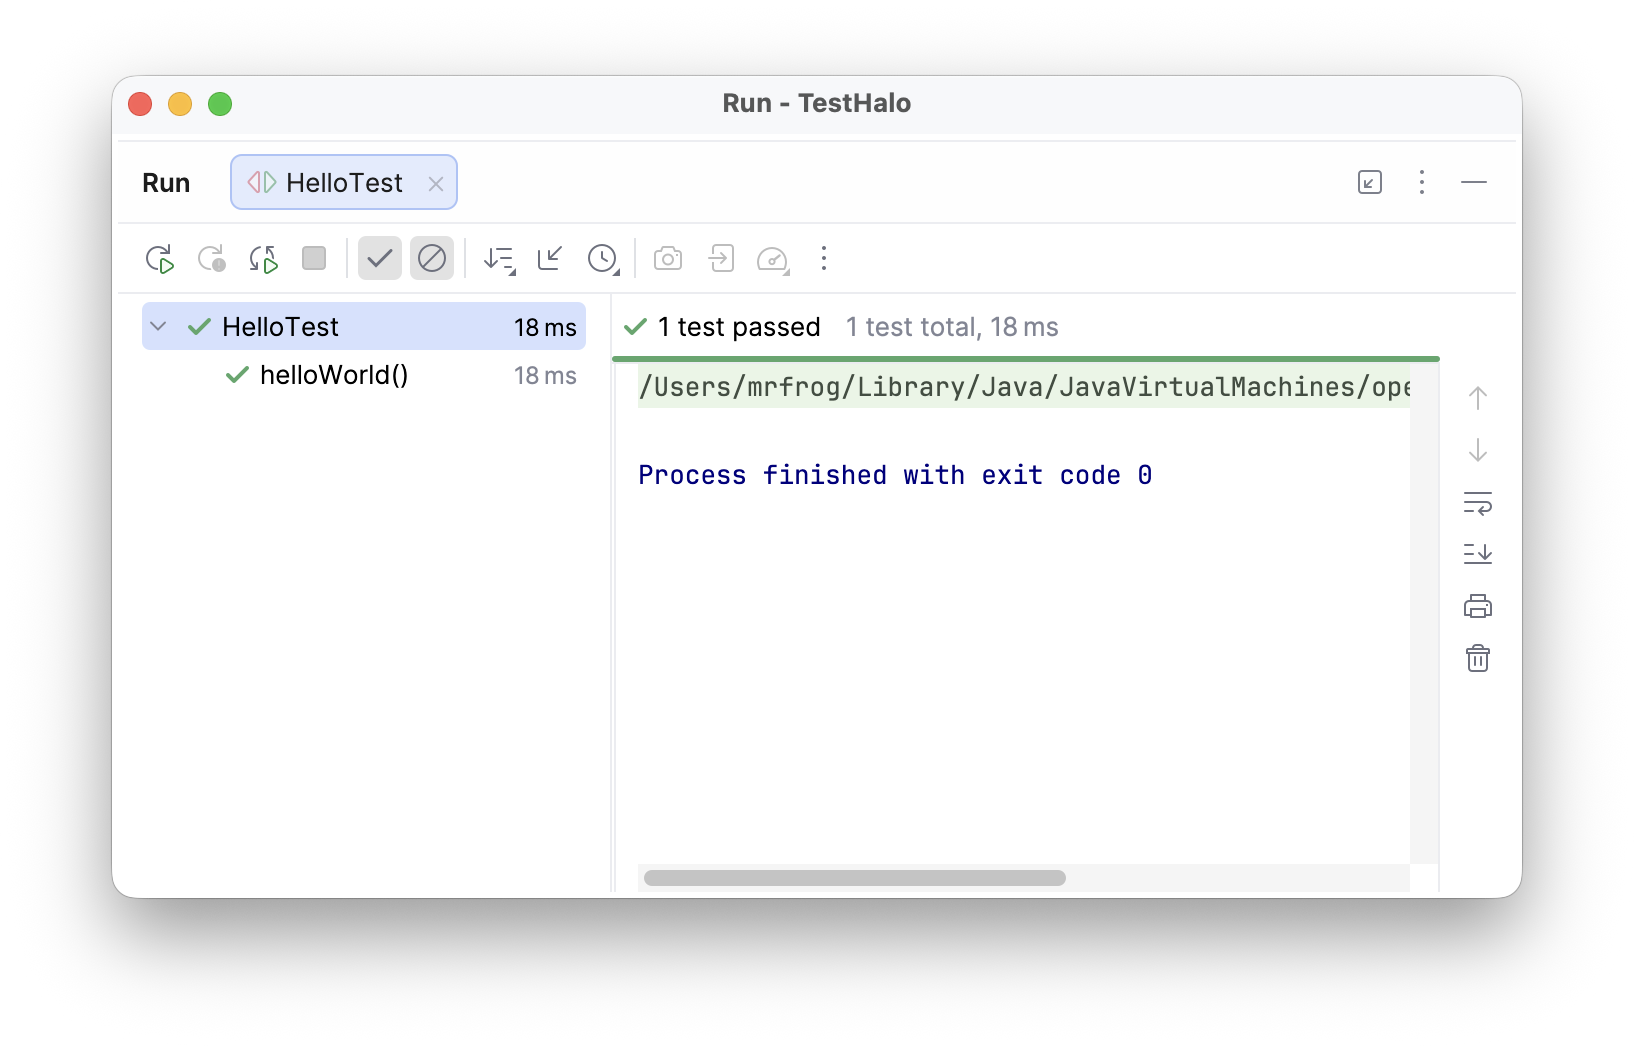
\includegraphics[width=0.7\textwidth]{hellotest.png}
        \caption{Hasil Unit Test Berhasil}
    \endfigure
\end{enumerate}
\section{Assertion}
\begin{enumerate}
    \item Buat class Java baru dengan nama \texttt{Calculator.java} pada folder \texttt{src/main/java} dengan isi sebagai berikut:
    \begin{lstlisting}[style=javastyle,caption=Contoh Class Calculator Java Sederhana]
public class Calculator {
    int a, b;

    public Calculator(int a, int b) {
        this.a = a;
        this.b = b;
    }

    public int tambah() {
        return a + b;
    }

    public int kurang() {
        return a - b;
    }

    public int bagi() {
        return a / b;
    }

    public int kali() {
        return a * b;
    }
}
\end{lstlisting} 
    \item Klik kanan pada nama class dan pilih show context actions, lalu pilih \texttt{Create Test} untuk membuat class test baru.
    \begin{figure}[H]
        \centering
        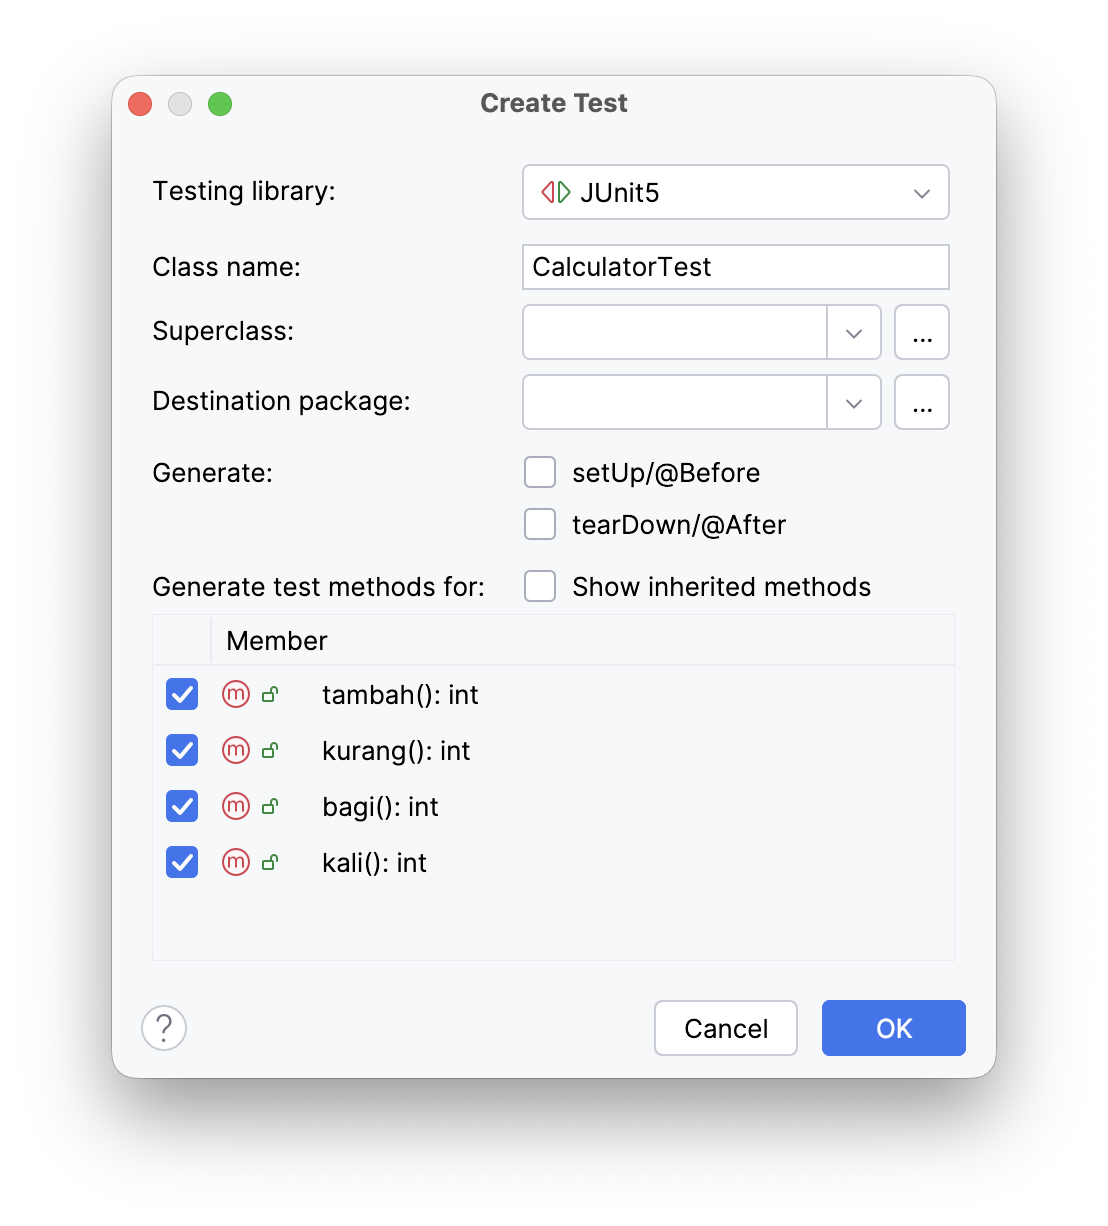
\includegraphics[width=0.7\textwidth]{createtest.png}
        \caption{Membuat Class Test dengan Context Actions}
    \end{figure}
    \item Pilih metode yang akan di test, lalu klik OK.
    \item Maka akan terbentuk class test baru, edit class test tersebut untuk menambahkan assertion pada setiap metode yang di test seperti berikut:
    \begin{lstlisting}[style=javastyle,caption=Contoh Class Test Calculator Java Sederhana]
// location: src/test/java/CalculatorTest.java
import org.junit.jupiter.api.Test;

import static org.junit.jupiter.api.Assertions.*;

class CalculatorTest {

    @Test
    void tambah() {
        Calculator Cal =  new Calculator(2,5);
        int actual = Cal.tambah();
        int expected = 7;

        assertEquals(actual,expected);
    }
\end{lstlisting}
\newpage
\begin{lstlisting}[style=javastyle,caption=Contoh Class Test Calculator Java Sederhana]
    @Test
    void kurang() {
        Calculator Cal = new Calculator(5, 2);
        int actual = Cal.kurang();
        int expected = 3;

        assertEquals(actual, expected);
    }

    @Test
    void bagi() {
        Calculator Cal = new Calculator(10, 2);
        int actual = Cal.bagi();
        int expected = 5;

        assertEquals(actual, expected);
    }

    @Test
    void kali() {
        Calculator Cal = new Calculator(3, 4);
        int actual = Cal.kali();
        int expected = 12;

        assertEquals(actual, expected);
    }
}
\end{lstlisting}
\item Jalankan class test untuk memastikan bahwa semua metode pada class \texttt{Calculator} telah diuji dengan benar.
\item Jika semua langkah di atas dilakukan dengan benar, maka hasil dari unit test akan menunjukkan bahwa semua test berhasil (green bar) seperti gambar berikut:
\begin{figure}[H]
    \centering
    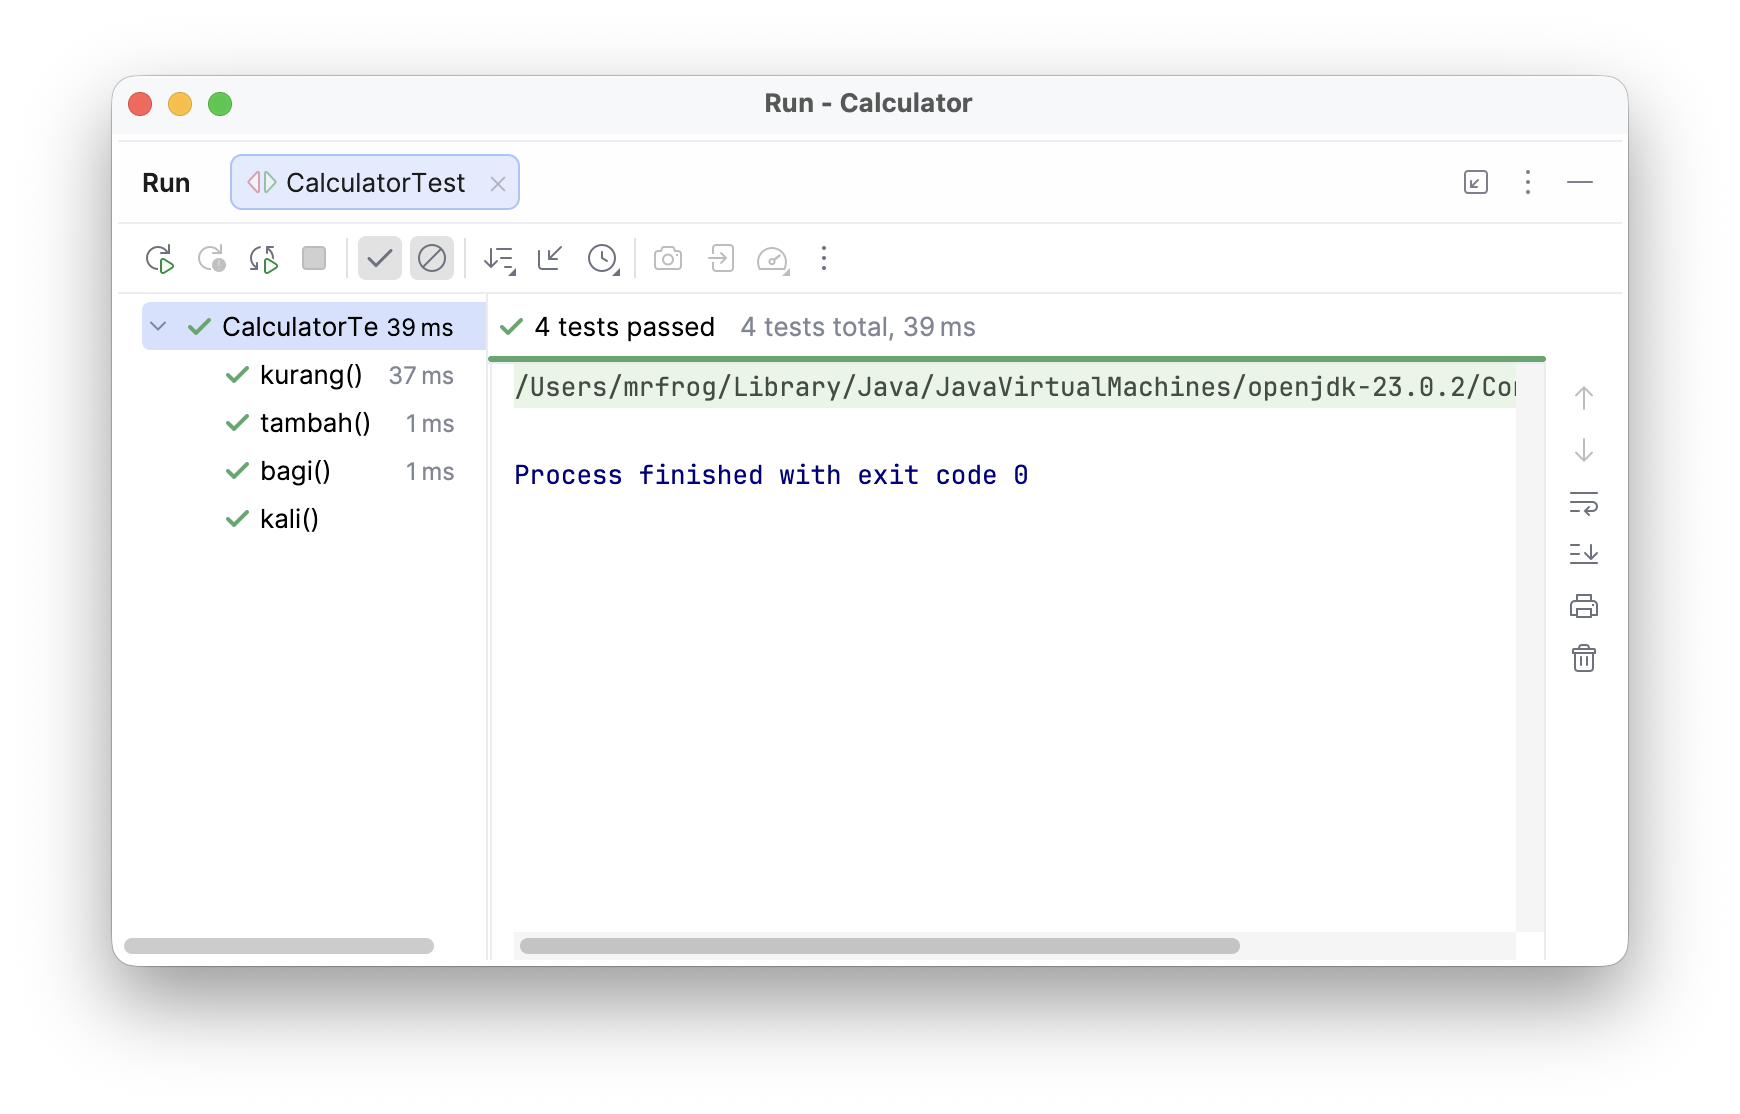
\includegraphics[width=0.7\textwidth]{calculatortest.png}
    \caption{Hasil Unit Test Calculator Berhasil}
\end{figure}


    
\end{enumerate}
\chapter{Tugas Praktikum}
\section{Unit Test}
\begin{enumerate}
    \item Buatlah sebuah kelas uji/test class yang berisi 2 test method. Method pertama menampilkan pesan "test class method 1" dan method ke-2 menampilkan pesan "test class method 2".
\begin{lstlisting}[style=javastyle,caption=Test Class dengan 2 Test Method]
// location: src/test/java/MyTestClass.java
import static org.junit.jupiter.api.Assertions.*;
import org.junit.jupiter.api.Test;

public class MyTestClass {
    @Test
    public void testMethod1() {
        System.out.println("test class method 1");
        assertTrue(true);
    }
    
    @Test
    public void testMethod2() {
        System.out.println("test class method 2");
        assertTrue(true);
    }
}
\end{lstlisting}
    
    \item Jalankan test class yang telah dibuat. berikut adalah hasil eksekusi dari test class tersebut:
    \begin{figure}[H]
        \centering
        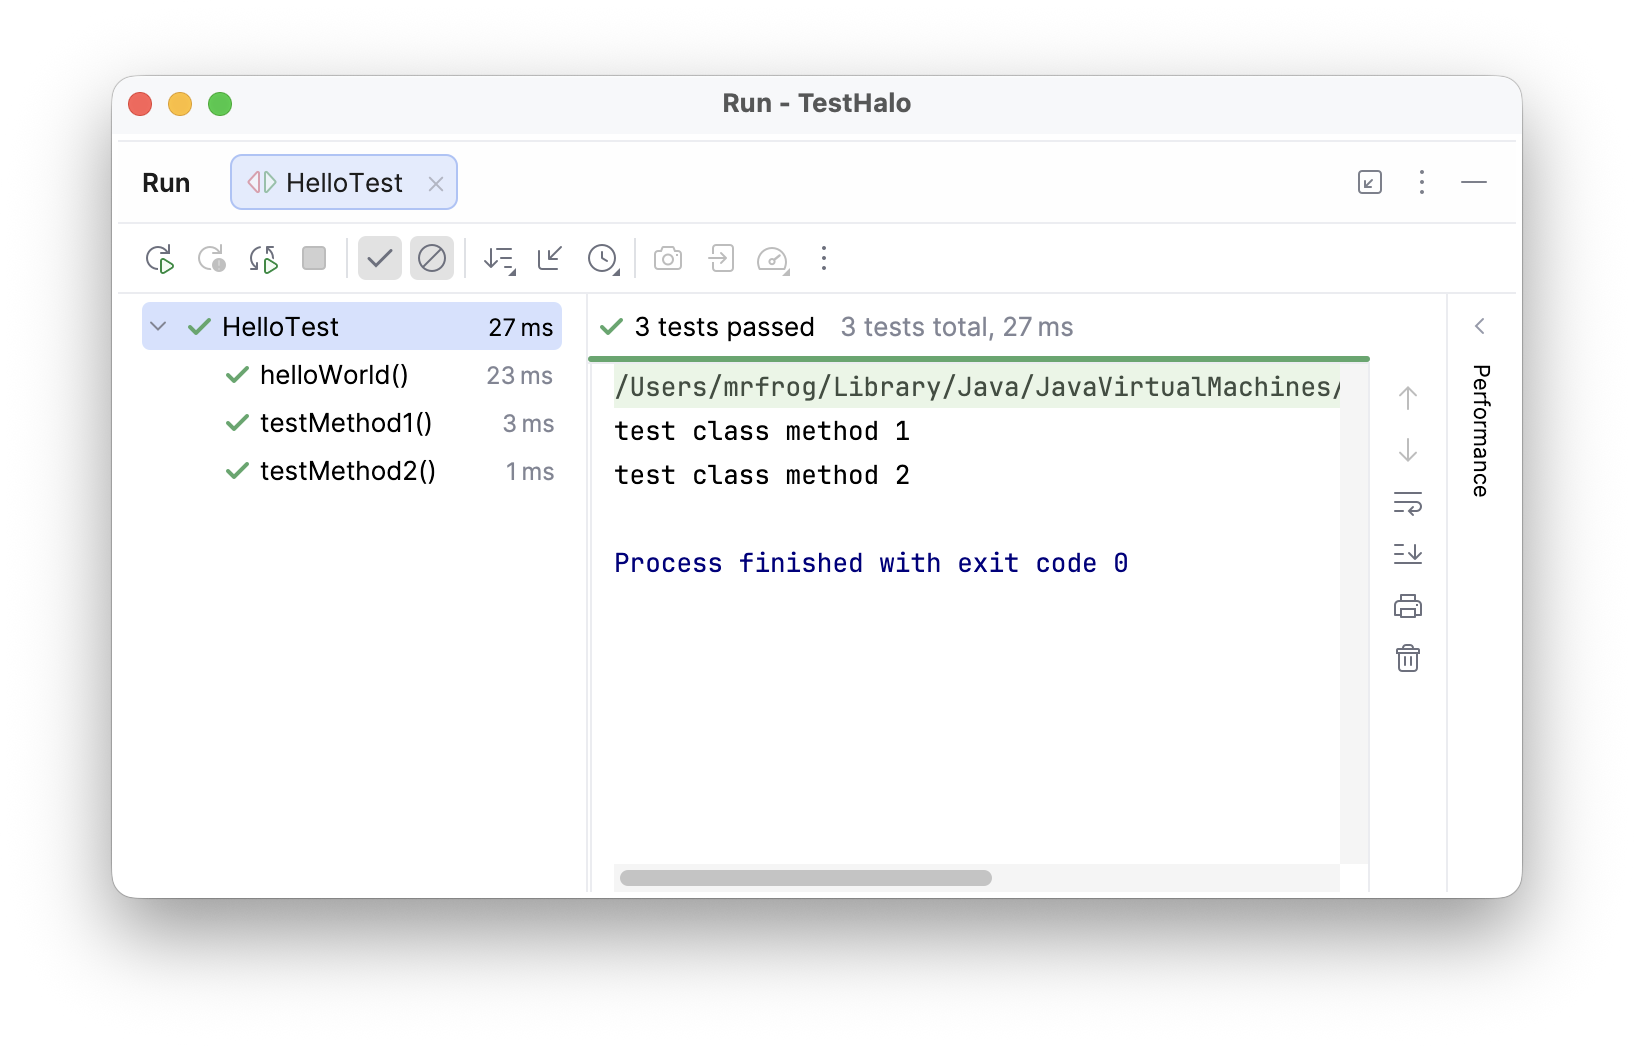
\includegraphics[width=0.7\textwidth]{testmethod.png}
        \caption{Hasil Eksekusi Test Class}
    \end{figure}
    
    \textbf{Hasil:} Kedua test method berhasil dijalankan dengan ditandai oleh green bar pada IDE. Output console menampilkan pesan dari masing-masing test method sesuai dengan yang diharapkan.
\end{enumerate}
\section{Assertion}
\begin{enumerate}
    \item Buatlah sebuah project baru dengan nama "Wallet" dengan Build System Maven, dan JUnit.
    \item Buatlah sebuah class bernama "Wallet" dengan atribut: owner, cards, totalMoney. Lalu buatlah methods untuk menambahkan kartu, mengambil kartu, menambahkan uang rupiah, mengambil uang, menampilkan jumlah uang yang ada di dompet. Berikut adalah contoh implementasi class Wallet:
\begin{lstlisting}[style=javastyle,caption=Class Wallet Sederhana]
// location: src/main/java/Wallet.java
import java.util.ArrayList;
import java.util.List;

public class Wallet {
    private String owner;
    private List<String> cards;
    private int totalMoney;

    public Wallet() {
        this.cards = new ArrayList<>();
        this.totalMoney = 0;
    }

    // set & get owner
    public void setOwner(String owner) {
        this.owner = owner;
    }

    public String getOwner() {
        return owner;
    }

    // kartu
    public void addCard(String card) {
        cards.add(card);
    }

    public String takeCard(String card) {
        if (cards.contains(card)) {
            cards.remove(card);
            return card;
        }
        return null;
    }

    public List<String> getCards() {
        return cards;
    }

    // uang
    public void addMoney(int amount) {
        if (amount > 0) {
            totalMoney += amount;
        }
    }

    public boolean takeMoney(int amount) {
        if (amount > 0 && totalMoney >= amount) {
            totalMoney -= amount;
            return true;
        }
        return false;
    }

    public int getTotalMoney() {
        return totalMoney;
    }

}
\end{lstlisting}
    \item Buat unit test untuk class Wallet dengan menggunakan berbagai macam assertion seperti berikut: 
\begin{lstlisting}[style=javastyle,caption=Class Test Wallet]
import org.junit.jupiter.api.BeforeEach;
import org.junit.jupiter.api.Test;

import static org.junit.jupiter.api.Assertions.*;

class WalletTest {

    Wallet wallet;

    @BeforeEach
    void setup() {
        wallet = new Wallet();
        wallet.setOwner("Janu");
    }

    @Test
    void testSetOwner() {
        assertEquals("Janu", wallet.getOwner());
    }

    @Test
    void testAddCard() {
        wallet.addCard("KTP");
        wallet.addCard("ATM");

        assertEquals(2, wallet.getCards().size());
        assertTrue(wallet.getCards().contains("KTP"));
    }

    @Test
    void testTakeCard() {
        wallet.addCard("SIM");
        String card = wallet.takeCard("SIM");

        assertNotNull(card);
        assertFalse(wallet.getCards().contains("SIM"));
    }

    @Test
    void testAddMoney() {
        wallet.addMoney(50000);
        wallet.addMoney(25000);

        assertEquals(75000, wallet.getTotalMoney());
    }

    @Test
    void testTakeMoney() {
        wallet.addMoney(100000);
        boolean result = wallet.takeMoney(40000);

        assertTrue(result);
        assertEquals(60000, wallet.getTotalMoney());
    }

    @Test
    void testWalletSummary() {
        wallet.addCard("ATM");
        wallet.addMoney(50000);

        assertAll(
                () -> assertEquals("Janu", wallet.getOwner()),
                () -> assertEquals(1, wallet.getCards().size()),
                () -> assertEquals(50000, wallet.getTotalMoney())
        );
    }
}
\end{lstlisting}
    \item Jalankan class test untuk memastikan bahwa semua metode pada class Wallet telah diuji dengan benar.
    \item Jika semua langkah di atas dilakukan dengan benar, maka hasil dari unit test akan menunjukkan bahwa semua test berhasil (green bar) seperti gambar berikut:
    \begin{figure}[H]
        \centering
        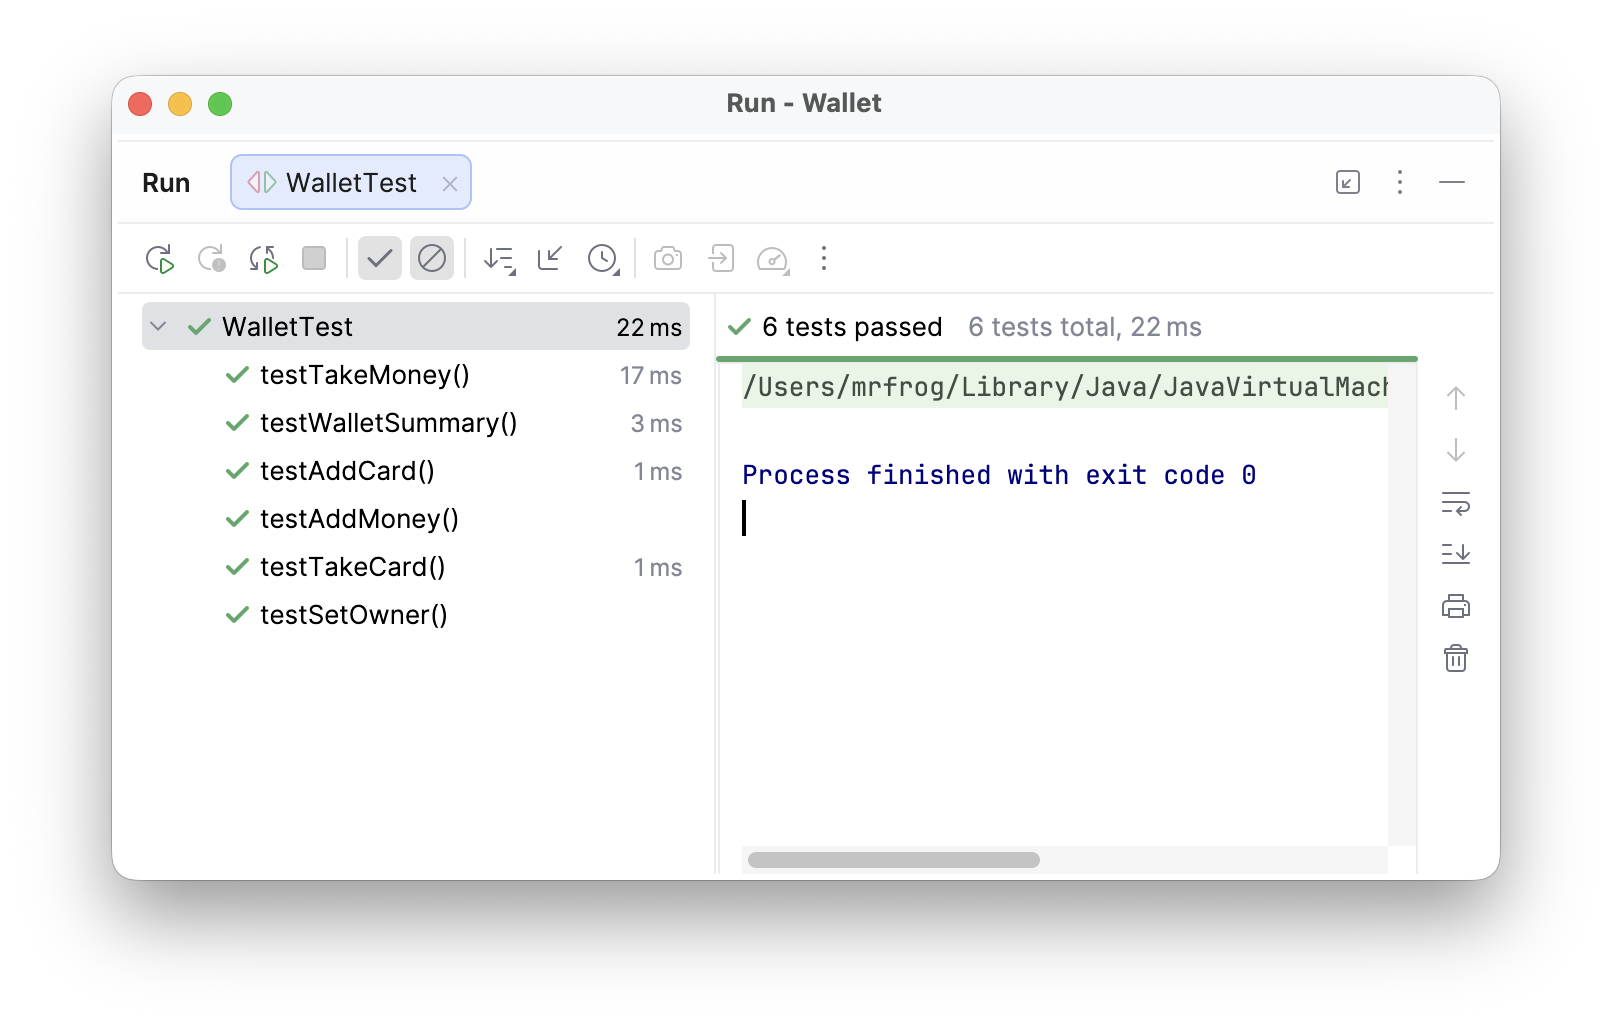
\includegraphics[width=0.7\textwidth]{wallettest.png}
        \caption{Hasil Unit Test Wallet Berhasil}
    \end{figure}
\end{enumerate}
\section*{Resources}
\url{https://github.com/januarsyah901/PPPL/tree/main/Pertemuan%201}
\chapter{Kesimpulan}
Dengan mempelajari dan mengimplementasikan unit test serta assertion menggunakan JUnit, mahasiswa dapat memahami pentingnya pengujian perangkat lunak dalam memastikan kualitas kode. Unit test membantu mendeteksi kesalahan lebih awal dalam proses pengembangan, sehingga meminimalkan risiko bug di kemudian hari. Selain itu, penggunaan assertion memungkinkan verifikasi hasil yang lebih akurat, memastikan bahwa fungsi-fungsi berjalan sesuai dengan yang diharapkan. Praktikum ini memberikan pengalaman praktis dalam menulis dan menjalankan unit test, yang merupakan keterampilan penting bagi pengembang perangkat lunak profesional.
\end{document}  